\chapter{Elementi di GRASS GIS}

\section{Informazioni generali%
%\footnote{GRASS GIS. (10 giugno 2009). Wikipedia, L'enciclopedia libera. Tratto il 26 agosto 2009, 15:41 da http://it.wikipedia.org/w/index.php?title=GRASS\_GIS\&oldid=24604028.}
}

	\begin{wrapfigure}{o}{0.35\columnwidth}
		\centering
		
\includegraphics[scale=0.15]{img/Grasslogo_vector_big}\par
		\caption{{\small Il logo di GRASS GIS.}}
	\end{wrapfigure}

	\textbf{GRASS} è l'acronimo di \textbf{G}eographic \textbf{R}esources \textbf{A}nalysis \textbf{S}upport \textbf{S}ystem. GRASS è un software libero di \emph{Geographical Information System} (GIS), rilasciato sotto la licenza GNU GPL. Esistono versioni per diverse piattaforme. GRASS nasce all'inizio degli anni '80 come progetto dell\textquoteright{}esercito degli Stati Uniti (\emph{US Army Corp of Engineering Research Laboratory} --- USACerl). Lo sviluppo avviene in particolare utilizzando il linguaggio C ed Unix come sistema operativo di riferimento. Nel 1996 l'esercito degli Stati Uniti prende la decisione di abbandonare lo sviluppo di GRASS. Gli utenti sono invitati a migrare verso sistemi commerciali, mentre l'ultima versione di GRASS (4.1) rimane nel pubblico dominio. Alla fine del 1997, dopo oltre un anno, riesce a formarsi un nuovo team internazionale che si fa carico di continuare lo sviluppo. L'aggiunta di nuovi moduli e porzioni di codice al software di pubblico dominio pone però il problema del diritto d'autore. Nell'ottobre 1999 dopo un'ampia discussione il GRASS Development Team (GDT) decide di rilasciare GRASS (5.0b) con la licenza GNU GPL. Attualmente il centro di sviluppo del software ha sede a Povo (Trento, Trentino --- Italia), presso l'ITC-irst, ma si avvale di molti collaboratori esterni. Il coordinatore del progetto è Markus Neteler.\\

	Tramite il sistema dei moduli, GRASS permette di utilizzare altri programmi quali

	\begin{description}
		\item [{PROJ.4}] libreria per le proiezioni cartografiche, usata in quasi i tutti i sistemi geografici liberi;
		\item [{OGR~Simple~Feature~Library}] gestione file vettoriali in diversi formati;
		\item [{GDAL}] (\emph{Geospatial Data Abstraction Library}), gestione file raster in diversi formati;
		\item [{R}] per gli aspetti statistici e di geostatistica.
	\end{description}
		
	GRASS GIS funziona sotto sistema operativo \emph{Unix} (o similari: GNU/Linux), sia su workstation che su personal computer e sotto sistema operativo \emph{Windows} mediante \emph{cygwin}, che simula l'ambiente Unix.


\section{Installazione su Ubuntu GNU/Linux\label{sec:Installazione-su-Ubuntu}}
	Questa guida è orientata all'utilizzo di GRASS su sistemi GNU/Linux, in particolare sulla distribuzione Ubuntu. Le seguenti indicazioni possono essere comunque applicate a qualsiasi distribuzione derivata da Debian GNU/Linux. Per ottenere GRASS è sufficiente installare i due pacchetti \texttt{grass} e \texttt{grass-doc}. È possibile farlo tramite terminale, con il comando \texttt{sudo apt-get install grass grass-doc} o tramite il gestore di pacchetti per GNOME, Synaptic. Per ulteriori informazioni su come installare software su Ubuntu si rimanda alla documentazione ufficiale della comunità italiana, presente online all'indirizzo \url{http://wiki.ubuntu-it.org/AmministrazioneSistema/InstallareProgrammi}. Si troverà anche molto utile l'installazione del software contenuto nel pacchetto \texttt{gdal-bin}.


\section{Caratteristiche principali\cite{uniparma}}

	\subsection{Gestione dei dati in GRASS}
		In GRASS ad ogni cella (pixel) che compone una carta raster, viene attribuito un solo valore di categoria ed eventualmente un'etichetta descrittiva. La non assegnazione di una categoria comporta l'assegnazione automatica di un valore particolare detto \emph{null}. La geometria di una carta vettoriale (uno dei due componenti oltre agli attributi) è riconducibile ad una delle cinque tipologie seguenti, che si discostano leggermente da quelle elencate precedentemente:
		
		\begin{description}
			\item [{point~(\emph{punto})}] per rappresentare gli elementi puntiformi (punti quotati, pozzi, ecc). Ogni punto è rappresentato da una coppia di coordinate.
			\item [{line~(\emph{linea})}] per rappresentare elementi lineari. Ogni linea è costituita da una \emph{spezzata}.
			\item [{boundary~(\emph{bordo})}] per rappresentare, anche parzialmente, i bordi di aree chiuse. È una spezzata memorizzata mediante una sequenza di coppie di coordinate in corrispondenza dei nodi e dei vertici.
			\item [{centroid~(\emph{centroide})}] è un elemento puntiforme all'interno di un'area chiusa in corrispondenza del quale vengono inseriti gli attributi dell'area; ogni centroide è rappresentato da una coppia di coordinate.
			\item [{area~(\emph{area})}] è l'insieme di un bordo di area (\emph{boundary}) completo (quindi chiuso) e del relativo centroide.
		\end{description}
		
		In GRASS, la geometria è salvata in un formato vettoriale specifico del programma (formato nativo), ma è comunque possibile importare e trasformare molti altri formati (ArcInfo-Coverages, CSV, SHAPE files, \emph{GIS ManagerL}, MapInfo, MySQL, ODBC, OGDI, PostgreSQL/PostGIS, S57, SDTS, TIGER, UK .NTF, VRT). Alcuni di questi formati (come lo shapefile) possono essere gestiti direttamente senza la conversione nel formato nativo. Come abbiamo considerato precedentemente, le informazioni vettoriali sono distinte nelle geometrie appena elencate e negli attributi. Geometrie ed attributi in GRASS vengono salvati separatamente in tabelle diverse, collegate tramite un valore univoco denominato \emph{cat}. Il collegamento tra geometrie ed attributi viene operato tramite una DBMI (\emph{DataBase Management Interface} -- Interfaccia di Gestione del DataBase). Attualmente GRASS gestisce i seguenti DBMI: DBF, PostgreSQL, MySQL, ODBC, mediante dei software interni (\emph{driver}), rispettivamente \emph{dbf}, \emph{pg} e \emph{ogr}. Il DBMI DBF è il driver di default: ciò significa che qualsiasi tipo di dato vettoriale importato in GRASS viene copiato dal software in una cartella di lavoro, e tutte le informazioni vengono trasferite in tabelle dbf in questa cartella. Vedremo in seguito com'è organizzata e come si gestisce la cartella di lavoro.\\

		La funzione della categoria (o colonna \emph{cat}) quindi è quella di fungere da {}``ponte'' tra le tabelle che contengono le coordinate geografiche dei vari punti che costituiscono le geometrie e gli attributi delle stesse geometrie, semplicemente conferendo agli attributi lo stesso valore di \emph{cat} delle geometrie che li presentano. La tabella \ref{tab:La-tabel} riassume questo concetto.

		\begin{table}
			\centering
			\input{tab/attributi}
			\qquad
			\input{tab/geometrie}
			\caption{\label{tab:La-tabel}{\small La tabella di sinistra sintetizza la struttura della tabella delle geometrie, contenente le coordinate dei punti e la loro topologia; la tabella a destra mostra come la colonna}\emph{\small cat}{\small{} determini il collegamento degli attributi (immagazzinati in un'apposita tabella) con le geometrie.}}
		\end{table}

		\input{tab/box_nomicarte}

	\subsection{Organizzazione dei dati}
		Una delle caratteristiche di GRASS rispetto ad altri software come Quantum GIS è l'estremo ordine con cui i dati vengono gestiti. Mentre la maggior parte dei software GIS si limita ad aprire i file mantenendoli nella loro posizione, quando un dato (di qualsiasi tipo) viene importato in GRASS, il programma ne crea una copia nella propria cartella di lavoro, elaborando i dati tramite il proprio driver predefinito (come precisato sopra, nella maggior parte dei casi il driver è il dbf). Con questa procedura automatica GRASS si crea automaticamente delle sottocartelle della propria cartella di lavoro, che può essere comunque posizionata a piacimento dell'utente su qualsiasi dispositivo (su una cartella in un PC locale o anche in un dispositivo di memorizzazione di massa come una penna USB). Comunque, in prima istanza, prima di poter operare, GRASS necessita che l'utente definisca una cartella ``radice'' in cui inserire tutti i dati. Nei sistemi operativi \emph{Unix} (come GNU/Linux) questa cartella viene posizionata in maniera predefinita nella \textsf{home} del sistema, per essere precisi nella cartella \textsf{grassdata} all'interno di \textsf{/home/nomeutente}. D'ora in poi assumeremo che la nostra cartella di lavoro sia appunto \textsf{/home/nomeutente/grassdata}.\\

		Esplorando il contenuto di una cartella di lavoro di GRASS, si noterà che essa è strutturata come nello schema \ref{tab:Organizzazione-schematica-della}.
		
		\begin{table}
			\begin{centering}
				\framebox{
					\begin{minipage}[t]{1\columnwidth}
						\dirtree{%
						.1 /home/nomeutente. 
						.2 grassdata. 
						.3 \underbar{location1}.\DTcomment{regione di lavoro}. 
						.4 PERMANENT.\DTcomment{mapset di base}. 
						.4 mapset1.\DTcomment{altri mapset$\downarrow$}. 
						.4 mapset2. 
						.4 mapset3. 
						.3 \underbar{location2}. 
						.4 PERMANENT. 
						.4 location1. 
						.4 location2. }
					\end{minipage}}
			\end{centering}
			\caption{{\small \label{tab:Organizzazione-schematica-della}Organizzazione schematica della cartella di lavoro di GRASS.}}
		\end{table}


		Le cartelle \textsf{location} sono create dall'utente, e rappresentano l'area su cui si intende operare. Per area è possibile considerare una qualsiasi estensione geografica (potenzialmente illimitata in estensione, sia in grande che in piccolo). Quindi, lavorando su uno scavo archeologico, una location potrebbe essere rappresentata dall'area di scavo, oppure --- parlando di uno scavo urbano d'emergenza --- dall'area dello scavo più l'area urbana nel raggio di 200 metri dal perimetro dello scavo. Anche le cartelle \textsf{mapset} vengono create dall'utente, e servono a immagazzinare le mappe. Non esiste alcun precetto che governi la gestione dei mapset, ma la loro struttura è tale da suggerire un utilizzo relativo ai tematismi: ogni tematismo va immagazzinato in un mapset. Dovendo gestire, ad esempio, un centinaio di tematismi, potrebbe comunque tornare utile unire più tematismi in un solo mapset.\\
		
		Un esempio pratico di come potrebbe essere organizzata una cartella di lavoro di GRASS all'interno di uno scavo archeologico è visibile nello schema \ref{tab:Organizzazione-schematica-della-1}.
		
		\begin{table}
			\begin{centering}
				\framebox{
					\begin{minipage}[t]{1\columnwidth}
						\dirtree{%
							.1 /home/nomeutente. 
							.2 grassdata. 
							.3 \underbar{siponto}.\DTcomment{regione di lavoro}. 
							.4 PERMANENT.\DTcomment{mapset di base}. 
							.4 idrografia.\DTcomment{altri mapset$\downarrow$}. 
							.4 edificato-medievale. 
							.4 tavoletta-IGM. 
							.4 prospezione-geofisica. 
							.3 \underbar{centro-storico-manfredonia}. 
							.4 PERMANENT. 
							.4 edificato-civile. 
							.4 strutture-muratura. }
					\end{minipage}}
			\end{centering}
			\caption{{\small \label{tab:Organizzazione-schematica-della-1}Esempio di organizzazione della cartella di lavoro di GRASS.}}
		\end{table}


		Ogni volta che viene creata una nuova location, viene automaticamente creato il mapset PERMANENT, che può essere modificato solo dal creatore della location\footnote{In GRASS è integrato il supporto all'utilizzo della stessa location da parte di molti utenti; questo ha portato alla necessità di definire delle regole per gestire le location, dando origine a mapset PERMANENT, che contiene le informazioni più importanti sulla location, e può essere modificata solo dall'utente che l'ha creata. Il problema comunque non si pone per installazioni in cui sia sempre lo stesso utente a fare il login nel sistema operativo.} e contiene diverse informazioni, come le coordinate della regione di lavoro e la risoluzione delle carte raster. Gli altri mapset della location sono creati dallo stesso o da altri utenti, in numero illimitato e con qualunque nome.

			\paragraph*{GRASS è ordinato\label{par:GRASS-=0000E8-ordinato}}
				Al contrario di molti software GIS e di tutti i CAD, GRASS è estremamente ordinato, sia nella gestione dei dati (come visto precedentemente) sia nell'importazione di questi. I dati con cui si lavora in un GIS, in particolare, sono divisibili in due categorie essenziali:
				
				\begin{description}
					\item [{dati~georeferenziati}] in questa descrizione ricadono tutti i dati (sia raster che vettoriali) i cui elementi che li compongono sono inseriti in un sistema di riferimento geografico; ciò significa che per ogni elemento (punto, linea, pixel, ecc.) è possibile esattamente conoscere la coordinata geografica.
					\item [{dati~non~georeferenziati}] sono tutti i dati i cui elementi non siano associabili a un sistema di riferimento geografico. In questa categoria possono ricadere sia le normali immagini TIFF o JPEG rappresentanti scansioni di mappe, sia i dati elaborati con un software CAD\footnote{In realtà il materiale elaborato tramite un CAD possiede un sistema di riferimento proprio, di tipo cartesiano, in cui ogni elemento viene posizionato in base ad una coppia di coordinate XY; tuttavia, l'impossibilità di associare ad una coordinata XY una coordinata geografica mette questi dati al pari di qualsiasi altro dato non georeferenziato.}.
				\end{description}
				
				L'approccio di GRASS alla gestione di queste due tipologie di dati risiede proprio nella creazione delle location: quando infatti l'utente decide di crearne una, deve \emph{necessariamente} specificare se la location dovrà contenere dati georeferenziati o no. Nel primo caso, sarà invitato dal programma a scegliere tutte le caratteristiche utili a definire il tipo di georeferenziazione (ad esempio il sistema di proiezione), per poter correttamente posizionare i dati georeferenziati all'interno della location\footnote{Adesso è più facile comprendere l'importanza del mapset PERMANENT, creato automaticamente insieme alla location, che conserva in alcuni file tutte le impostazioni della location, tra cui anche il sistema di riferimento.}. Nel secondo caso, l'utente dovrà importare i dati in una location caratterizzata dal cosiddetto \textsf{Arbitrary non-earth coordinate system (XY)} ovvero un sistema di coordinate arbitrario basato su una coppia di assi cartesiani $xy$ all'interno dei quali i dati della location verranno posizionati. Quindi, in GRASS è impossibile utilizzare la stessa location per dati georeferenziati e non georeferenziati, ma è possibile georeferenziare i dati di una location XY e ``muovere'' i dati elaborati in una location georeferenziata.


	\subsection{Comandi e documentazione}
		Tutta la documentazione ufficiale sull'utilizzo di GRASS è compresa nel \emph{GRASS Reference Manual} consultabile liberamente online\footnote{\href{http://grass.itc.it/grass60/manuals/html60_user/index.html}{http://grass.itc.it/grass60/manuals/html60\_{}user/index.html}}, in cui sono descritti tutti i comandi offerti dal software. Ricordando che GRASS è strutturato in moduli, si è aiutati nella memorizzazione dei comandi dal fatto che la lettera iniziale di ogni comando richiama la tipologia di dato su cui si va ad operare. Alcuni esempi sono visibili in tab.~\ref{tab:Esempi-di-comandi}. Fortunatamente per gli utenti che si avvicinano per la prima volta a GRASS, lo sforzo mnemonico è stato notevolmente ridotto dall'introduzione delle interfacce grafiche e dei menù, dai quali la stragrande maggioranza dei comandi e dei moduli del software sono accessibili tramite un nome descrittivo, senza necessità di imparare a memoria il comando\footnote{Tuttavia, nel processo di gestione consapevole dei dati, è sempre bene conoscere quale comando e quindi quale modulo ci sia dietro l'operazione che si sta compiendo, per questo motivo in questo manualetto faremo riferimento sia alla voce di menù sia al nome del comando.}.\\

		I moduli possono essere richiamati quindi indifferentemente sia attraverso le voci di menù sia digitando il comando che avvia il modulo nella finestra di terminale che è aperta contemporaneamente all'interfaccia grafica di GRASS. In seguito approfondiremo questo argomento.

		\input{tab/comandi_grass}

\section{Primi passi}

	\subsection{\label{sub:Avviare-GRASS-GIS}Avviare GRASS GIS: le interfacce}
		In una normale installazione su sistemi operativi GNU/Linux, GRASS non è avviabile da alcun menù o icona sul desktop, ma deve essere avviato da terminale. Su Ubuntu GNU/Linux, è necessario avviare il terminale tramite il menù \textsf{$\text{Applicazioni}\rightarrow\text{Accessori}\rightarrow\text{Terminale}$}. Sono disponibili varie interfacce grafiche per lavorare con GRASS, che pur essendo essenzialmente simili tra loro, possono apparire più o meno gradevoli a seconda dell'aspetto e dell'organizzazione dei menù. A chi usa per la prima volta GRASS si consiglia in qusta sede l'utilizzo dell'interfaccia realizzata con il linguaggio di programmazione wxPython, che rappresenta un buon compromesso tra funzionalità ed estetica. Per dovere di cronaca si ricorda tuttavia che alternative altrettanto valide possono essere sia l'interfaccia scritta in Tcl/Tk sia l'utilizzo di Quantum GIS come interfaccia a GRASS (quest'ultimo argomento verrà approfondito nell'appendice \ref{cha:Usare-QGIS-come}).\\

		Per avviare GRASS con interfaccia wxPython, è sufficiente far seguire al comando di avvio (\texttt{grass64}) il nome dell'interfaccia preceduta da un trattino (\texttt{-}).\\

		Digitare quindi \texttt{grass64 -wxpython} e premere \textsf{Invio}.\footnote{Nel \textsection\ref{des:Definireun'interfacciagraficadidefault} verrà spiegato come semplificare questo passaggio per i successivi avvii di GRASS.}\\

		Ci verrà presentata una finestra in cui sono elencate sulla sinistra tutte le location (\textsf{Project location}), e sulla destra tutti i mapset (\textsf{Accessible mapsets}) della location selezionata; queste caselle dovrebbero al momento essere vuote, essendo la prima volta che avviamo GRASS. Nella parte alta della finestra è presente una casella di testo in cui inserire (o selezionare sfogliandolo) il percorso per la nostra cartella di lavoro di GRASS (\textsf{grassdata}). Come visto precedentemente, si consiglia di posizionarla nella nostra home (\textsf{/home/nomeutente/grassdata}).


	\subsection{Definire una \emph{location\label{sub:Definire-una-location}}}
		Prima di creare una location, dobbiamo essere a conoscenza dei seguenti parametri:
		
		\begin{itemize}
			\item sistema di coordinate (cartesiano XY oppure proiezione, ellissoide e datum);
			\item area d'interesse (coordinate minime e massime dell'area di lavoro);
			\item risoluzione del raster (ovvero pixel di altezza e larghezza del raster, se si intende importare un raster; si veda \textsection\ref{sec:Importare-una-carta}).
		\end{itemize}
		
		All'estrema destra della finestra, nella box \textsf{Manage} sono presenti i pulsanti che permettono di gestire le location ed i mapset. Per cominciare, creiamo una nuova location premendo il pulsante \textsf{Location wizard}.


			\paragraph{Proiezioni e datum}
				Si presume che in questo contesto si voglia lavorare con il sistema di coordinate \emph{Universal Transverse Mercator} (UTM, la cui proiezione è la \emph{trasversale di Mercatore}) con datum WGS84\input{cap/foot_WGS}, quindi con un sistema di coordinate definito da latitudine e longitudine. Esistono una serie enorme di altri sistemi di proiezione (tutti supportati da GRASS), alcuni studiati per applicazioni specifiche, tra cui il ``vecchio'' Cassini (utilizzato in Italia nel XIX secolo) e il noto Gauss-Boaga (tutt'ora il sistema di proiezione ufficiale per la cartografia italiana). Un approfondimento sulle proiezioni e sui sistemi di riferimento può essere trovato nell'appendice \textsection\ref{cha:Proiezioni}. Citando Paolo Zatelli\footnote{\href{http://www.ing.unitn.it/~zatelli/cartografia_numerica/slides/SistRif_in_GRASS.pdf}{http://www.ing.unitn.it/$\sim$zatelli/cartografia\_{}numerica/slides/SistRif\_{}in\_{}GRASS.pdf}}:
				
				\begin{quotation}
					La necessità di definire un \emph{sistema di riferimento} è legata al carattere intrinsecamente relativo del concetto di posizione (la posizione ``rispetto a'' qualcosa), definendo il sistema di riferimento si indica rispetto a cosa sono date le coordinate. La \emph{proiezione} indica invece come si passa da posizioni sull'ellissoide di rotazione usato per definire il sistema di riferimento al piano della carta: questi due aspetti sono concettualmente distinti ed indipendenti ma nella pratica si devono sempre usare assieme. Per questo motivo vengono sempre definiti assieme e la trasformazione tra sistemi di riferimento è in realtà spesso una trasformazione tra sistemi di riferimenti e sistemi di proiezione diversi allo stesso tempo. Non trattiamo gli aspetti teorici della definizione e trasformazione di sistemi di riferimento e proiezione, di cui esiste ampia letteratura, ma solo della loro implementazione in GRASS.
				\end{quotation}
				
				Nella finestra appena aperta ci verrà chiesto di definire un nome per la nuova location; inserirlo nell'apposita casella di testo e premere \textsf{Next}. Adesso occorre definire il sistema di coordinate.  Possiamo scegliere tra le seguenti opzioni:
				
				\begin{description}
					\item [{\textsf{Select~coordinate~system}}] permette di scegliere manualmente tipo di proiezione, datum ed ellissoide;
					\item [{\textsf{Select~EPSG~code~of~coordinate~system}}] permette di scegliere il codice EPSG\footnote{L'\emph{European Petroleum Survey Group}, è stata un'organizzazione scientifica (il cui ciclo vitale si è chiuso nel 2005) legata all'industria del petrolio formata da esperti in geodesia, rilievo e cartografia, legati all'estrazione di idrocarburi; tale organizzazione ha compilato e diffuso il database \emph{EPSG Geodetic Parameter Set}, comprendente una serie di codici che identificano precisi ellissoidi di riferimento, datum geodetici, sistemi di coordinate geografiche e proiettati, unità di misura, ecc. per le varie nazioni e aree del pianeta. I codici EPSG vengono utilizzati per impostare velocemente questi parametri mentre si lavora in sistemi GIS; ad esempio, il codice EPSG del sistema WGS84 è il 4326 mentre quelli per i sistemi Gauss-Boaga adottati in Italia sono 3003 per il fuso Ovest e 3004 per il fuso Est.} che identifica il sistema geodetico di riferimento;
					\item [{\textsf{Use~coordinate~system~of~selected~georeferenced~file}}] permette di caricare un file già georeferenziato del quale conosciamo la bontà e di usare gli stessi parametri di quel file per impostare la nuova location;
					\item [{\textsf{Use~coordinate~system~of~selected~WKT~or~PRJ~file}}] permette di caricare le impostazioni da un file WKT o PRJ già in nostro possesso\footnote{I file PRJ sono associati agli SHAPE file (esattamente al pari dei file con estensione \emph{shp}, \emph{shx}, \emph{dbf}) e conservano le informazioni relative alla proiezione ed al sistema di riferimento impiegato nello SHAPE.};
					\item [{\textsf{Create~custom~PROJ.4~parameters~string~for~coordinate~system}}] permette di scrivere manualmente un file delle impostazioni utilizzando il linguaggio fornito dalla libreria di proiezioni cartografiche PROJ.4;
					\item [{\textsf{Use~arbitrary~non-earth~coordinate~system~(XY)}}] definisce una location caratterizzata da un sistema di riferimento cartesiano XY, utile per importare dati non georeferenziati.
				\end{description}
				
				Le opzioni solitamente più utili per chi non ha particolari esigenze sono quelle di importare un file PRJ da uno SHAPEfile già in nostro possesso e che contiene già i parametri del sistema WGS84, oppure se si ha a disposizione un raster georeferenziato si possono prelevare le impostazioni tramite la terza opzione. In generale, il contenuto di un file PRJ (modificabile con qualsiasi editor di testo) può essere simile al seguente (su una sola riga, viene qui spezzato):
				
				{\small\begin{verbatim}
						GEOGCS[``GCS_WGS_1984'',DATUM[``D_WGS\_1984'',
						SPHEROID[``WGS_1984'',6378137,298.257223563]],
						PRIMEM[``Greenwich'',0],UNIT[``Degree'',0.017453292519943295]]
					\end{verbatim}}
				
				Procediamo quindi premendo \textsf{Next} e proseguiamo durante la procedura guidata fino all'ultimo passaggio (solitamente chiamato \textsf{Summary}) dove premendo \textsf{Finish} avremo terminato di impostare la location. Prima di poter avere accesso alla finestra principale, GRASS chiederà se impostare una regione di default per la location definita.

				\input{tab/box_codici_epsg}

	\subsection{Definire una \emph{region}}
		Considerato che la location di lavoro impostata è attualmente semplicemente un sistema di riferimento senza dati, nasce la necessità di definire una \emph{region}, che è una regione di lavoro rettangolare che identifica la regione geografica (definita dalle coordinate dei bordi del rettangolo), all'interno della quale hanno effetto le operazioni eseguite da GRASS.  La regione deve essere definita in concomitanza con la creazione di una location e viene assunta come regione di default. Tale regione non può essere modificata ed è sempre disponibile. È tuttavia possibile definire altre regioni durante una sessione di GRASS, che possono essere salvate e richiamate in qualunque momento\footnote{Durante i primi utilizzi di GRASS, è comune non avere ben chiari i concetti di \emph{regione}, \emph{estensione della mappa} e \emph{area di visualizzazione}. Ad esempio, avendo a disposizione una mappa o dei dati molto estesi, è probabile che si voglia concentrare l'analisi in una zona più ristretta: per far ciò si imposta la \emph{regione} indicando i limiti spaziali di tale zona, accompagnata dalla \emph{risoluzione} dei dati (solitamente 1 pixel; la risoluzione della mappa di partenza può essere diversa da quella della regione). Come si vedrà successivamente, all'interno della finestra di visualizzazione della mappa, è possibile effettuare uno \emph{zoom}, concentrando l'attenzione su un'area ancora più ristretta della regione: in tal caso sarà cambiata l'\emph{area di visualizzazione}.}. Quindi, prima di poter accedere alla finestra principale, è possibile rispondere \textsf{si} o \textsf{no} alla richiesta di definire una \emph{region}. Rispondendo affermativamente verrà visualizzata una finestra in cui è possibile indicare le coordinate degli estremi dell'area che vogliamo importare successivamente; rispondendo negativamente ritorneremo alla finestra principale, e sarà comunque possibile definire la region successivamente in fase di importazione dei dati.\\

		Per avviare GRASS nella location appena creata, selezionarla dalla casella a sinistra e premere il pulsante \textsf{Start GRASS} in basso. Appariranno due finestre, il GIS Manager (il titolo della finestra è \textsf{GRASS GIS Layer Manager}) ed il \textsf{GRASS GIS Map Display}; inoltre, il terminale da cui abbiamo precedentemente avviato GRASS restituirà un output simile a quello riportato in fig.~\ref{fig:Output-del-terminale}, offrendoci anche la possibilità adesso di accedere alla riga di comando.
		
		\begin{figure}
			\centering
			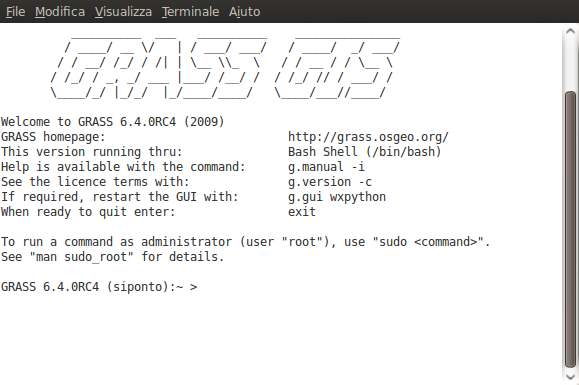
\includegraphics[scale=0.4]{img/screenshot_001}
			\caption{{\small \label{fig:Output-del-terminale}Output del terminale una volta avviato GRASS.}}
		\end{figure}

		Dal GIS Manager è possibile accedere a quasi tutte le funzioni di GRASS, ivi compresa l'eventuale prima definizione o modifica della \emph{region}; è possibile farlo dal menù \textsf{$\text{Config}\rightarrow\text{Region}\rightarrow\text{Set~region}$}. La finestra che si aprirà ci permetterà, nella scheda \textsf{Bounds} di impostare tramite 4 coordinate i 4 limiti del rettangolo di lavoro (nelle prime quattro box della scheda). Le coordinate devono essere inserite nel formato \textsf{AA:MM:SS\{N|S\}}\footnote{Angolo:Minuti:Secondi; le parentesi graffe non devono essere inserite.}, lasciando vuote tutte le altre box di testo; al termine, premere \textsf{Run}. Ad esempio, la regione del sito archeologico di Siponto medievale risponde alle seguenti coordinate:
		
		{\small\begin{verbatim}
			north: 42:00:01N
			south: 40:59:58N
			west: 14:59:59E
			east: 16:00:01E
			\end{verbatim}}
		
		\input{tab/box_interrogare_sisrif}

	\subsection{Usare Layer Manager e Map Display}
		Una volta avviato GRASS in una certa location, le due finestre principali su cui si lavora sono proprio il Layer Manager ed il Map Display (visibili in fig.~\ref{fig:Da-sinistra,-Layer}); il primo permette di controllare quasi tutte le funzioni di GRASS; in linea generale, ogni azione selezionabile dai vari menù del Layer Manager corrisponde ad un modulo di GRASS, ovvero un software che svolge una certa funzione, che è avviabile anche da terminale (esattamente come si è visto per il modulo di definizione della regione, \textsf{g.region} che è utilizzabile sia da riga di comando che dall'interfaccia tramite menù). Sia il Layer Manager che il Map Display fanno capo ad un unico modulo di GRASS, \textsf{g.gui} (si ricordi infatti che il prefisso \textsf{g.} identifica proprio una funzione generale del programma). Si provi infatti a chiudere entrambe le finestre, mantenendo il terminale aperto: la riga di comando ci ricorda in che location è attualmente situato GRASS (il nome è tra parentesi). Sarà sufficiente dare il comando \texttt{g.gui} per ottenere nuovamente Layer Manager e Map Display per la location corrente.
		
		\begin{figure}
			\centering
			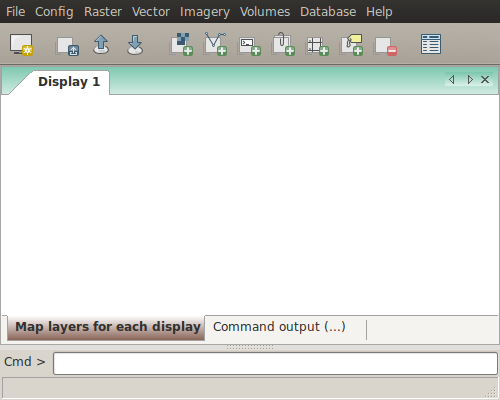
\includegraphics[scale=0.31]{img/screenshot_003}
			\qquad{}
			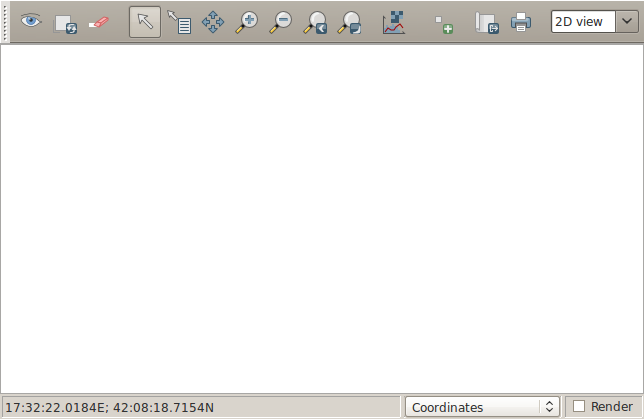
\includegraphics[scale=0.3]{img/screenshot_002}
			\caption{{\small \label{fig:Da-sinistra,-Layer}Da sinistra, Layer Manager e Map Display.}}
		\end{figure}

		\begin{description}
			\item [{Layer~Manager}] come da nome, è il gestore dei layer di GRASS per la location aperta; i layer vengono elencati nella sua scheda principale (visibile in basso, nominata \textsf{Map layers for each display}), mentre nella seconda scheda, \textsf{Command output} si può leggere l'output di testo che ogni comando aperto dal Layer Manager scrive, sia che il comando sia andato a buon fine che in caso contrario.  È molto importante, in caso d'errore, leggere il contenuto di \textsf{Command output}, perché fornisce chiari riferimenti alla natura dell'errore. Il Layer Manager, pur essendo gestito tramite menù, permette di conoscere il nome del comando associato ad ogni voce di menù: è sufficiente spostare il puntatore su una voce per osservare nel bordo inferiore della finestra, il comando associato a quella voce; riprendendo quanto fatto precedentemente, posizionando il cursore su \textsf{$\text{Config}\rightarrow \text{Region}\rightarrow \text{Set~region}$} si leggerà nella casella a piede del Layer Manager la dicitura \texttt{g.region -p} che è il comando da terminale che avvia la scelta della region. Tale funzione può risultare utile per memorizzare progressivamente i nomi dei moduli e la loro funzione.
				
				\begin{description}
					\item [{\label{des:Definireun'interfacciagraficadidefault}Definire~un'interfaccia~grafica~di~default}] È possibile definire un'interfaccia grafica per GRASS in maniera definitiva, senza doverla specificare nel comando di avvio nel terminale. Per farlo, selezionare \textsf{$\text{Config}\rightarrow \text{GRASS~working~enviroment}\rightarrow \text{Change~default~GUI}$}. Dal menù a tendina \textsf{GUI~type} della scheda \textsf{Required} selezionare \textsf{wxpython} e poi \textsf{Run}. D'ora in poi l'interfaccia predefinita per avviare GRASS sarà quella selezionata, ed il programma potrà essere avviato semplicemente con il comando \texttt{grass64} anziché \texttt{grass64 -wxpython} (come visto precedentemente in \textsection\ref{sub:Avviare-GRASS-GIS}).
					\item [{Salvare~le~impostazioni~dell'area~di~lavoro}] Dopo aver caricato certi layer all'interno del Layer Manager, ed aver definito alcune loro caratteristiche (opacità, posizione), è probabile voler salvare lo stato delle cose per poterlo riottenere tale in un secondo momento; le impostazioni possono essere salvate tramite \textsf{$\text{File}\rightarrow \text{Workspace}\rightarrow \text{Save~as}$} in un file, che potrà essere caricato in caso di necessità con \textsf{$\text{File}\rightarrow \text{Workspace}\rightarrow \text{Load}$}. Si raccomanda di salvare tale file nella cartella \textsf{grassdata}.
				\end{description}
			
			\item [{Map~Display}] è associato al Layer Manager e ne visualizza i contenuti. È dotato, da sinistra verso destra, di pulsanti che permettono di renderizzare la mappa da zero, aggiornare la mappa (dopo aver operato piccoli cambiamenti sui layer), cancellare il rendering della mappa, selezionare il puntatore, interrogare la mappa, muovere la mappa, aumentare e diminuire lo zoom, ritornare all'ultimo zoom usato. Il decimo pulsante da sinistra, \textsf{Zoom options}, offre delle funzioni avanzate, tra cui lo zoom sulla mappa attualmente selezionata nel Layer Manager, la possibilità di zoomare sulla region di default (precedentemente definita), di zoomare ad una region salvata con un certo nome, o di salvare l'estensione visualizzata correntemente con un nuovo nome. Il pulsante successivo \textsf{Analyze} offre la possibilità di visualizzare dei grafici di analisi relativi alla mappa corrente, ed in particolare la distanza tra due punti, il profilo di superficie e un istogramma del file raster. Segue il pulsante \textsf{Add overlay} con cui è possibile aggiungere delle caratteristiche aggiuntive alla mappa, utili per la stampa: la barra di scala e la freccia del Nord, una legenda o un layer di testo da riempire a discrezione dell'utente. I due pulsanti successivi \textsf{Save display to PNG file} e \textsf{Print display} permettono rispettivamente di esportare e di stampare la mappa. L'ultimo pulsante è un menù a tendina dal quale è possibile selezionare il tipo di rendering della mappa (3D o 3D; \textsf{digitize} identifica la modalità di \emph{editing}, che sarà spiegata in seguito). È importante notare che nella parte bassa del Map Display è presente un menù a tendina che permette di definire quali valori debbano essere visualizzati: in default il menù è impostato sulla visualizzazione delle coordinate del puntatore, ma è possibile anche selezionare la visualizzazione statica dell'estensione della regione (\textsf{Extent}), della regione computazionale (\textsf{Comp. region}) e relativa estensione (\textsf{Show comp. extent}), informazioni sulla geometria e sulla scala della mappa.
		\end{description}
